% !TEX root = ../../prj4projektrapport.tex
% SKAL STÅ I TOPPEN AF ALLE FILER FOR AT MASTER-filen KOMPILERES 

\section{Kontrolmodul}

Kontrolmodulet består af en Siemens PLC S7-1200 med signalmodulet AQ1x12BIT. Det kan tilgås gennem en switch af typen CSM 1277.
Softwaren består af to dele; en kommunikationsdel med interface til kommunikationsmodulet og en kontroldel med interface til Trinskifter. Den detaljerede gennemgang af softwaren kan findes i dokumentationen.\footnote{Projektdokumentation, 10.1, Kontrolmodul} Her vil i stedet blive lagt fokus på de overvejelser, der har været undervejs i designet af Kontrolmodulet.
Kontrolmodulet er lavet i en OB, der looper. Heri er placeret fire FC'er, der er oprettet i forbindelse med kommunikationen og den FB, der er fremstillet til styring af Trinskifter.

\subsection{Kommunikation}
Datatransmission til Kontrolmodulet er en vigtig del af projektet, da dette forbinder sensorer i form af Måleenhederne med aktuatorer i form af Trinskifter. Derfor er der blevet lagt mange overvejelser i, hvordan kommunikationen skulle etableres.


Først og fremmest skulle flere Måleenheder kunne kommunikere med det samme kontrolmodul, derfor var en switch i overvejelser, grundet der kun er én fri RJ-45 port på PLC'en. Dette var ikke umiddelbart muligt at fremskaffe hos værkstedet. For mere om løsningerne på dette, se afsnit \ref{Kommunikationsmodul}.


Næste beslutning gik på valget af protokol til Ethernet kommunikation. TCP var det oplagte valg for at sikre pålidelig kommunikation, selvom UDP også var en kendt protokol fra faget Internet kommunikationsnetværk(IKN).


Udvilingsværktøjet TIA Portal V13 har gode muligheder for at sætte TCP kommunikation op til forskellige ikke Siemens produkter gennem dets open user communication. Først blev blokkene TSEND\_C og TRCV\_C forsøgt anvendt. Disse blokke har dog indbygget funktionalitet i forbindelse med at oprette og nedlægge forbindelsen, hvilket var uhensigtmæssigt, når der skulle være en flydende datastrøm. Det endelige valg blev derfor blokkene TCON, TDISCON, TSEND og TRCV, hvor man som programmør kan styre oprettelse og nedlæggelse af forbindelsen med TCON og TDISCON. På figur \ref{fig:TSEND} ses blokken TSEND som et eksempel på open user communication blokkene.

\begin{figure}[H] % (alternativt [H])
	\centering
	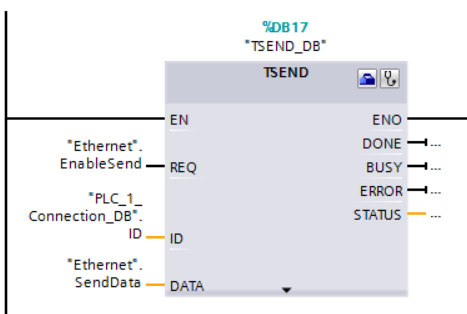
\includegraphics[width=0.5\textwidth]{Figure/TSEND}
	\caption{Blokken TSEND}
	\label{fig:TSEND}
\end{figure}


Med en pålidelig og testet TCP kommunikation var de næste overvejelser angående styringen af disse blokke. Her blev det besluttet, at et client/server forhold ville være bedst. Kontrolmodulet er i den sammenhæng client og skal forespørge data fra serveren, Kommunikationsmodulet.
Da systemet ikke er et beskyttelsessystem, kræver det ikke hurtig reaktion mellem sensor og aktuator. Derfor blev det valgt, at det kun var nødvendigt at opdatere data hvert 2 sekunder. Dette blev realiseret med to separate netværk; et tilknyttet FC'en med TSEND og et tilknyttet FC'en med TRCV. På figur \ref{fig:ValgAfEnhedSend} ses netværket tilknyttet TSEND.

\begin{figure}[H] % (alternativt [H])
	\centering
	\includegraphics[width=1\textwidth]{Figure/valgAfEnhedSend}
	\caption{Netværket der styrer hvilken enhed der forespørges data fra}
	\label{fig:ValgAfEnhedSend}
\end{figure}

FC'er er valgt, da tanken var at hukommelsen skulle ligge andetsteds i koden. Det er dog blevet nødvendigt at oprette en global DB for at kunne styre variable i forbindelse med styring af kommunikationen. For yderlige uddybelse, se dokumentationen\footnote{Projektdokumentation, 10.1.1, TCP kommunikation}.


Det er vigtigt at pointere, at systemet skal være nemt at udvide til at understøtte mange Måleenheder i den virkelige verden. Det vil udvide tiden, det tager at eksekvere programmet, men er nemt, da der ikke skal ændres i selve kommunikationen, men kun i de netværk, der styrer kommunikationen, hvor der her skal tilføjes flere forgreninger.

\subsection{Styring af Trinskifter}

Angående styring af Trinskifteren blev det tidligt besluttet at benytte dens analoge 24VDC udgange på Q0.6, Q0.7 og Q1.0 til styringen af relæerne på Trinskifter. Disse udgange bliver dog styret med et logisk højt (24VDC) eller lavt(0V) signal. Der henvises til Trinskifter for mere om relækredsløbet, se afsnit \ref{sec:relae}.
Samtidig er projektet proof of concept, så det er kun spændingsmålinger fra én forbruger, der vil blive reguleret med hensyn til. Dette simplificerer den FB, der udvikles til denne styring væsentligt, da der kun er et input. På \ref{fig:GraphTrinskifterPLC} ses et diagram over sekvenserne og flowet imellem dem for FB'en Trinskifter.

\begin{figure}[H] % (alternativt [H])
	\centering
	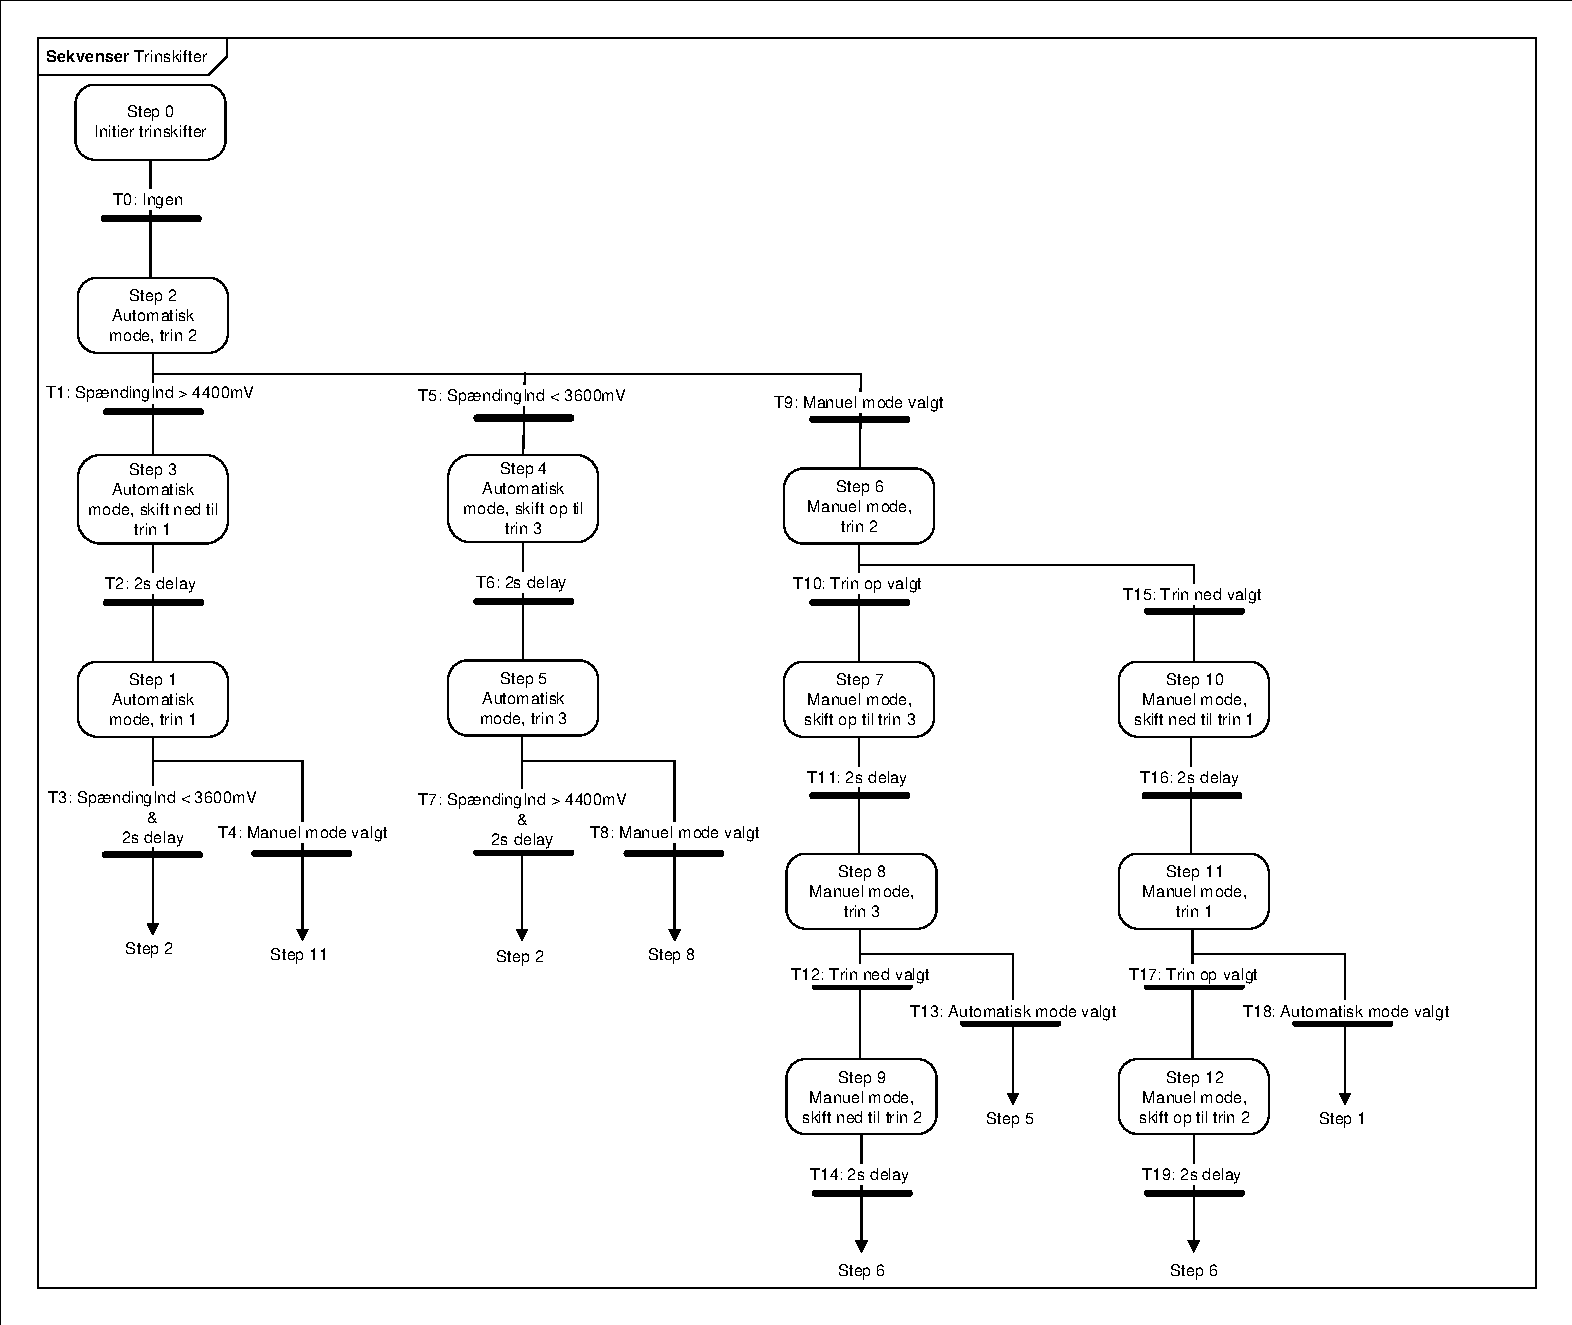
\includegraphics[width=1\textwidth]{Figure/GraphTrinskifterPLC}
	\caption{Diagrammet viser FB'en Trinskifters sekvenser}
	\label{fig:GraphTrinskifterPLC}
\end{figure}

Første tanke i forhold til denne blok var, at den hovedsageligt skulle være automatiseret. Derfor er det besluttet, at koden blev skrevet som sekventiel, hvor en lokal static Step står for at styre, hvilken sekvens der er aktiv. Dette sikrer også imod fejl, da systemet har få muligheder videre fra hvert step. Et sikkert system var også et af de vigtige punkter, hvilket bl.a. er opnået ved at opdele koden i sekvenser af trin og trinskift. Der er 3 trin, som hver især er tilknyttet en af udgangene på PLC'en. For trin 2 er der både mulighed for et trinskift op og ned, mens der for ydertrinene kun kan skiftes ned/op til trin 2. Det er kun, når koden er i et trin, at man kan skifte mellem automatisk og manuel tilstand. I automatisk mode er der dog to undtagelser i trin 1 og trin 3, hvor trinskiftet er lagt sammen med trinet. Disse trinskift burde have været flyttet til deres egen sekvens for at undgå at et trinskift og et tilstandsskift kan forekomme samtidigt.


I første udkast til blokken var der ikke taget højde for at programmet blev eksekveret hurtigere end data blev opdateret, derfor kunne programmet nå at skifte flere trin på den samme måling, hvilket vil skabe et ustabilt system, for når det havde lavet et dobbeltskift, vil det så få en ny måling, der indikerer skift i modsat retning. Denne fejl er fjernet ved at indsætte et delay, når systemet kommer i et nyt trin, da der hentes ny data hvert 2 sekunder, er dette delay sat til 2,5 sekunder.


En vigtig pointe at få med er, at forbrugeren aldrig må miste forsyning. Så et trinskift indebærer et overlap imellem de trin, der skiftes fra og til på 2 sekunder. Herved er der altid forsyning på distributionslinjen. Selve overlappet set fra trintransformeren uddybes i afsnit \ref{sec:ImpTrinskift}.
For mere om styringen af trinskifteren, se dokumentationen.\footnote{Projektdokumentation, 10.1.2, Styring af Trinskifteren.}
